% !TEX root = ../notes_unsupervisedlearning.tex
% Chapter 3: Hierarchical Clustering
%%%%%%%%%%%%%%%%%%%%%%%%%%%%%%%%%%%%%%%%%%%%%%%%%%%%%%%%%%%%%%%%%%%%%%

\chapter{Hierarchical Clustering}\index{Hierarchical Clustering}\index{Dendrogram}
\newthought{Structure exists at multiple scales.}

%═══════════════════════════════════════════════════════════════════════
% BLOCK 1: INTRODUCTION
%═══════════════════════════════════════════════════════════════════════

\section{The Why}

\marginnote{Hierarchies are everywhere: taxonomies, organizational charts, file systems, evolutionary trees.}

K-Means asks: "What are the $K$ groups?" But often we don't know $K$, and structure exists at multiple resolutions. Consider:

\begin{itemize}
    \item \textbf{Biology}: Species $\subset$ Genus $\subset$ Family $\subset$ Order $\subset$ Class $\subset$ Phylum $\subset$ Kingdom
    \item \textbf{Geography}: Neighborhood $\subset$ District $\subset$ City $\subset$ Region $\subset$ Country
    \item \textbf{Documents}: Sentences $\subset$ Paragraphs $\subset$ Sections $\subset$ Chapters $\subset$ Books
\end{itemize}

\textbf{Hierarchical clustering} produces a tree structure (dendrogram) that captures all levels of grouping simultaneously. You can cut the tree at any height to get a flat clustering.

\subsection{Hands-On Experience}

\begin{marginfigure}
\begin{tikzpicture}[scale=0.6]
    \begin{axis}[
        xlabel={$x_1$},
        ylabel={$x_2$},
        xmin=0, xmax=10,
        ymin=0, ymax=4,
        width=\textwidth,
        height=0.6\textwidth,
    ]
    \addplot[only marks, mark=*, mark size=3pt, blue] coordinates {
        (1,1) (2,1) (3,1) (6,2) (7,2) (9,3)
    };
    \node[anchor=north] at (axis cs:1,1) {A};
    \node[anchor=north] at (axis cs:2,1) {B};
    \node[anchor=north] at (axis cs:3,1) {C};
    \node[anchor=north] at (axis cs:6,2) {D};
    \node[anchor=north] at (axis cs:7,2) {E};
    \node[anchor=north] at (axis cs:9,3) {F};
    \end{axis}
\end{tikzpicture}
\caption{Six points for hierarchical clustering.}
\end{marginfigure}

Consider six points: $A=(1,1)$, $B=(2,1)$, $C=(3,1)$, $D=(6,2)$, $E=(7,2)$, $F=(9,3)$.

\textbf{Build a dendrogram by hand} using single linkage (minimum distance):

\begin{enumerate}
    \item Initial distances: $d(A,B)=1$, $d(B,C)=1$, $d(D,E)=1$ (smallest)
    \item Merge A-B at height 1
    \item Merge D-E at height 1 (tie)
    \item Now $d(\{A,B\}, C) = \min(d(A,C), d(B,C)) = 1$
    \item Merge \{A,B\}-C at height 1
    \item Continue until all points are merged...
\end{enumerate}

The result is a tree showing nested structure: $\{A,B,C\}$ and $\{D,E\}$ form tight groups, with $F$ joining later.

\subsection{Learning Objectives}

After this lecture, you will be able to:
\begin{enumerate}
    \item Distinguish between agglomerative and divisive hierarchical clustering
    \item Apply different linkage criteria (single, complete, average, Ward's)
    \item Construct and interpret dendrograms
    \item Choose appropriate cutting strategies to extract flat clusterings
    \item Analyze computational complexity trade-offs
\end{enumerate}

%═══════════════════════════════════════════════════════════════════════
% BLOCK 2: MAIN THEORY
%═══════════════════════════════════════════════════════════════════════

\section{Agglomerative Clustering}

\marginnote{Bottom-up: start with each point as its own cluster, merge closest pairs.}

\textbf{Agglomerative} (bottom-up) clustering is the most common approach:

\begin{algorithm}[H]
\caption{Agglomerative Hierarchical Clustering}
\begin{algorithmic}[1]
\Require Data $X = \{x_1, \ldots, x_n\}$, linkage criterion $L$
\Ensure Dendrogram $T$
\State Initialize: each point is its own cluster $C_i = \{x_i\}$
\State Compute pairwise distances $D[i,j] = d(C_i, C_j)$
\While{more than one cluster remains}
    \State Find $(i^*, j^*) = \arg\min_{i \neq j} D[i,j]$
    \State Record merge: $(C_{i^*}, C_{j^*})$ at height $D[i^*, j^*]$
    \State Create new cluster $C_{\text{new}} = C_{i^*} \cup C_{j^*}$
    \State Update distances to $C_{\text{new}}$ using linkage $L$
    \State Remove $C_{i^*}$ and $C_{j^*}$ from active clusters
\EndWhile
\end{algorithmic}
\end{algorithm}

The key choice is the \textbf{linkage criterion}: how do we measure distance between clusters?


\section{Linkage Criteria}

\marginnote{Different linkages produce very different dendrograms.}

Let $C_i$ and $C_j$ be two clusters. The distance $D(C_i, C_j)$ depends on linkage:

\subsection{Single Linkage (Minimum)}

\begin{equation}
    D_{\text{single}}(C_i, C_j) = \min_{x \in C_i, y \in C_j} d(x, y)
\end{equation}

\textbf{Properties}:
\begin{itemize}
    \item Can find non-convex, elongated clusters
    \item Suffers from \textbf{chaining}: single close points can bridge distant clusters
    \item Sensitive to noise and outliers
\end{itemize}

\subsection{Complete Linkage (Maximum)}

\begin{equation}
    D_{\text{complete}}(C_i, C_j) = \max_{x \in C_i, y \in C_j} d(x, y)
\end{equation}

\textbf{Properties}:
\begin{itemize}
    \item Produces compact, roughly equal-diameter clusters
    \item Robust to chaining
    \item May break apart natural elongated clusters
\end{itemize}

\subsection{Average Linkage (UPGMA)}

\begin{equation}
    D_{\text{average}}(C_i, C_j) = \frac{1}{|C_i| |C_j|} \sum_{x \in C_i} \sum_{y \in C_j} d(x, y)
\end{equation}

\marginnote{UPGMA: Unweighted Pair Group Method with Arithmetic Mean}

\textbf{Properties}: Compromise between single and complete linkage.

\subsection{Ward's Method}

Merge clusters that minimize the increase in total within-cluster variance:

\begin{equation}
    D_{\text{Ward}}(C_i, C_j) = \frac{|C_i| |C_j|}{|C_i| + |C_j|} \|\mu_i - \mu_j\|^2
\end{equation}

where $\mu_i$ and $\mu_j$ are cluster centroids.

\marginnote{Ward's method is equivalent to K-Means in some sense---it minimizes variance.}

\textbf{Properties}:
\begin{itemize}
    \item Produces compact, spherical clusters (like K-Means)
    \item Often gives the most "intuitive" results for Euclidean data
    \item Only works with Euclidean distance
\end{itemize}

\begin{figure}[h]
\centering
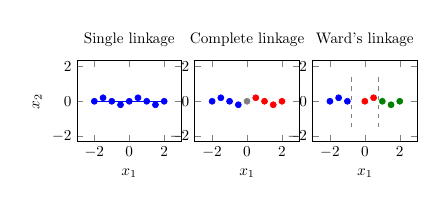
\begin{tikzpicture}[scale=0.55]
    % Single linkage
    \begin{axis}[
        name=single,
        title={Single linkage},
        xlabel={$x_1$}, ylabel={$x_2$},
        xmin=-3, xmax=3, ymin=-2, ymax=2,
        width=0.33\textwidth,
        axis equal,
    ]
    % Chain-like data
    \addplot[only marks, mark=*, mark size=2pt, blue] coordinates {
        (-2,0) (-1.5,0.2) (-1,0) (-0.5,-0.2) (0,0)
        (0.5,0.2) (1,0) (1.5,-0.2) (2,0)
    };
    \draw[blue, thick] (axis cs:-2,0) -- (axis cs:2,0);
    \end{axis}

    % Complete linkage
    \begin{axis}[
        at={(single.east)}, anchor=west, xshift=0.3cm,
        name=complete,
        title={Complete linkage},
        xlabel={$x_1$},
        xmin=-3, xmax=3, ymin=-2, ymax=2,
        width=0.33\textwidth,
        axis equal,
    ]
    \addplot[only marks, mark=*, mark size=2pt, blue] coordinates {
        (-2,0) (-1.5,0.2) (-1,0) (-0.5,-0.2)
    };
    \addplot[only marks, mark=*, mark size=2pt, red] coordinates {
        (0.5,0.2) (1,0) (1.5,-0.2) (2,0)
    };
    \addplot[only marks, mark=*, mark size=2pt, gray] coordinates {(0,0)};
    \end{axis}

    % Ward's linkage
    \begin{axis}[
        at={(complete.east)}, anchor=west, xshift=0.3cm,
        title={Ward's linkage},
        xlabel={$x_1$},
        xmin=-3, xmax=3, ymin=-2, ymax=2,
        width=0.33\textwidth,
        axis equal,
    ]
    \addplot[only marks, mark=*, mark size=2pt, blue] coordinates {
        (-2,0) (-1.5,0.2) (-1,0)
    };
    \addplot[only marks, mark=*, mark size=2pt, red] coordinates {
        (0,0) (0.5,0.2)
    };
    \addplot[only marks, mark=*, mark size=2pt, green!50!black] coordinates {
        (1,0) (1.5,-0.2) (2,0)
    };
    \draw[gray, dashed] (axis cs:-0.75,-1.5) -- (axis cs:-0.75,1.5);
    \draw[gray, dashed] (axis cs:0.75,-1.5) -- (axis cs:0.75,1.5);
    \end{axis}
\end{tikzpicture}
\caption{Same data, different linkages, different clusters. Single linkage chains; complete/Ward split into compact groups.}
\end{figure}


\section{The Dendrogram}

\marginnote{A dendrogram is a tree diagram showing hierarchical relationships.}

The \textbf{dendrogram} visualizes the entire clustering hierarchy:

\begin{figure}[h]
\centering
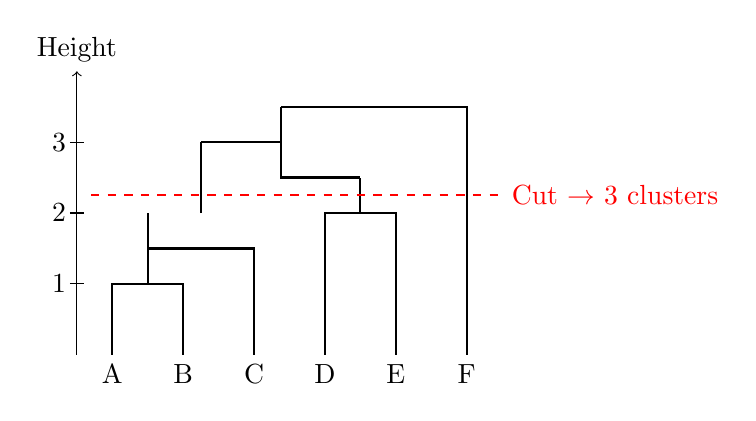
\begin{tikzpicture}[scale=0.9]
    % Dendrogram
    \draw[thick] (0,0) -- (0,1) -- (1,1) -- (1,0);
    \draw[thick] (0.5,1) -- (0.5,2);
    \draw[thick] (2,0) -- (2,1.5) -- (0.5,1.5) -- (0.5,2);
    \draw[thick] (1.25,2) -- (1.25,3);
    \draw[thick] (3,0) -- (3,2) -- (4,2) -- (4,0);
    \draw[thick] (3.5,2) -- (3.5,2.5);
    \draw[thick] (1.25,3) -- (2.375,3) -- (2.375,2.5) -- (3.5,2.5);
    \draw[thick] (5,0) -- (5,3.5) -- (2.375,3.5);
    \draw[thick] (2.375,3) -- (2.375,3.5);

    % Labels
    \node[anchor=north] at (0,0) {A};
    \node[anchor=north] at (1,0) {B};
    \node[anchor=north] at (2,0) {C};
    \node[anchor=north] at (3,0) {D};
    \node[anchor=north] at (4,0) {E};
    \node[anchor=north] at (5,0) {F};

    % Height axis
    \draw[->] (-0.5,0) -- (-0.5,4) node[anchor=south] {Height};
    \foreach \y in {1,2,3} {
        \draw (-0.6,\y) -- (-0.4,\y) node[anchor=east, xshift=-3pt] {\y};
    }

    % Cut line
    \draw[red, dashed, thick] (-0.3,2.25) -- (5.5,2.25);
    \node[red, anchor=west] at (5.5,2.25) {Cut $\to$ 3 clusters};
\end{tikzpicture}
\caption{Dendrogram showing hierarchical structure. Cutting at height 2.25 yields 3 clusters: $\{A,B,C\}$, $\{D,E\}$, $\{F\}$.}
\label{fig:dendrogram}
\end{figure}

\textbf{Reading a dendrogram}:
\begin{itemize}
    \item \textbf{Leaves}: Individual data points (bottom)
    \item \textbf{Internal nodes}: Cluster merges
    \item \textbf{Height}: Distance at which clusters merged
    \item \textbf{Horizontal cut}: Produces a flat clustering (more clusters at lower cuts)
\end{itemize}

\subsection{Cophenetic Correlation}

\marginnote{Cophenetic correlation measures how well the dendrogram preserves original distances.}

The \textbf{cophenetic distance} $c(i,j)$ is the height at which points $i$ and $j$ first merge. The cophenetic correlation:
\begin{equation}
    r_{\text{coph}} = \text{corr}(d(i,j), c(i,j))
\end{equation}
measures how faithfully the dendrogram represents the original distance matrix. Higher is better (max = 1).


\section{Cutting the Dendrogram}

To get a flat clustering, we must \textbf{cut} the dendrogram. Several strategies:

\subsection{Cut at Fixed Height}

Choose a distance threshold $h$; all merges above $h$ are cut:
\begin{equation}
    K = \#\{\text{branches crossing height } h\}
\end{equation}

\subsection{Cut for Fixed Number of Clusters}

Find the height $h$ that gives exactly $K$ clusters.

\subsection{Dynamic Cutting}

\marginnote{Dynamic cutting adapts to local tree structure.}

The \textbf{inconsistency} coefficient compares a merge height to its subtree:
\begin{equation}
    I(m) = \frac{h(m) - \bar{h}_{\text{sub}}}{\sigma_{h,\text{sub}}}
\end{equation}

Cut where inconsistency exceeds a threshold (default: 0.7--0.9).


\section{Divisive Clustering}

\marginnote{Top-down: start with all points, recursively split.}

\textbf{Divisive} (top-down) clustering works in reverse:

\begin{algorithm}[H]
\caption{Divisive Hierarchical Clustering (DIANA)}
\begin{algorithmic}[1]
\State Start with all points in one cluster
\While{not all points are singletons}
    \State Select cluster with largest diameter/variance
    \State Split it into two sub-clusters (e.g., using K-Means with $K=2$)
\EndWhile
\end{algorithmic}
\end{algorithm}

\textbf{Comparison}:
\begin{itemize}
    \item Agglomerative: $O(n^2)$ to $O(n^3)$ time, focuses on local similarities
    \item Divisive: More expensive, but can use global information for splits
\end{itemize}


\section{Computational Complexity}

\marginnote{Naive hierarchical clustering is $O(n^3)$---prohibitive for large datasets.}

\begin{table}[h]
\centering
\begin{tabular}{lcc}
\toprule
\textbf{Algorithm} & \textbf{Time} & \textbf{Space} \\
\midrule
Naive agglomerative & $O(n^3)$ & $O(n^2)$ \\
Single linkage (SLINK) & $O(n^2)$ & $O(n)$ \\
Complete/Average & $O(n^2 \log n)$ & $O(n^2)$ \\
BIRCH (approximate) & $O(n)$ & $O(n)$ \\
\bottomrule
\end{tabular}
\caption{Computational complexity of hierarchical clustering algorithms}
\end{table}

For large datasets ($n > 10,000$), consider:
\begin{itemize}
    \item \textbf{BIRCH}: Build a CF-tree, then cluster the tree nodes
    \item \textbf{Sampling}: Cluster a sample, assign remaining points
    \item \textbf{Approximate methods}: HDBSCAN, etc.
\end{itemize}


%═══════════════════════════════════════════════════════════════════════
% BLOCK 3: STUDENT ACTIVATION
%═══════════════════════════════════════════════════════════════════════

\section{Examples \& Exercises}

\subsection{Exercise 1: Dendrogram Construction}

Given the distance matrix:

\begin{table}[h]
\centering
\begin{tabular}{c|cccc}
 & A & B & C & D \\
\hline
A & 0 & 2 & 6 & 10 \\
B & 2 & 0 & 5 & 9 \\
C & 6 & 5 & 0 & 4 \\
D & 10 & 9 & 4 & 0 \\
\end{tabular}
\end{table}

Build a dendrogram using single linkage.

\textbf{Solution}:
\begin{enumerate}
    \item Smallest distance: $d(A,B) = 2$. Merge A-B at height 2.
    \item Update distances: $d(\{A,B\}, C) = \min(6,5) = 5$, $d(\{A,B\}, D) = \min(10,9) = 9$
    \item Smallest: $d(C,D) = 4$. Merge C-D at height 4.
    \item Remaining: $d(\{A,B\}, \{C,D\}) = \min(5,9,6,4) = 4$... wait, we need to recalculate.
    \item $d(\{A,B\}, \{C,D\}) = \min(d(A,C), d(A,D), d(B,C), d(B,D)) = \min(6,10,5,9) = 5$
    \item Merge \{A,B\}-\{C,D\} at height 5.
\end{enumerate}

Dendrogram: A-B merge at 2, C-D merge at 4, then merge at 5.

\subsection{Exercise 2: Linkage Comparison}

Using the same distance matrix, build dendrograms with complete linkage and compare.

\textbf{Solution}:
\begin{enumerate}
    \item Merge A-B at height 2 (same)
    \item $d_{\text{complete}}(\{A,B\}, C) = \max(6,5) = 6$
    \item $d_{\text{complete}}(C,D) = 4$ (smallest). Merge C-D at height 4.
    \item $d_{\text{complete}}(\{A,B\}, \{C,D\}) = \max(6,10,5,9) = 10$
    \item Final merge at height 10.
\end{enumerate}

Complete linkage merges the two groups much later (height 10 vs 5), reflecting the maximum inter-cluster distance.

\subsection{Exercise 3: Cutting Strategies}

For the dendrogram from Exercise 1, determine:
\begin{enumerate}
    \item The clustering if we cut at height 3
    \item The clustering if we want exactly 2 clusters
\end{enumerate}

\textbf{Solution}:
\begin{enumerate}
    \item At height 3: \{A,B\} is formed (merged at 2), but C-D not yet merged (height 4). Result: \{A,B\}, \{C\}, \{D\} = 3 clusters.
    \item For 2 clusters: cut between heights 4 and 5. Result: \{A,B\}, \{C,D\}.
\end{enumerate}


\section{Self-Reflection \& Recap}

\subsection{Reflection Questions}
\begin{enumerate}
    \item Why does single linkage tend to produce "chaining"?
    \begin{quote}
        \textit{Single linkage only requires one close pair to merge clusters. A chain of nearby points can progressively connect distant groups, even if most points in the groups are far apart.}
    \end{quote}

    \item When would you prefer Ward's linkage over complete linkage?
    \begin{quote}
        \textit{Ward's method produces more balanced, spherical clusters and works well when clusters have similar sizes. It's the default choice for Euclidean data when you expect compact clusters.}
    \end{quote}

    \item How do you decide where to cut a dendrogram?
    \begin{quote}
        \textit{Look for large gaps (long vertical lines without branches), use domain knowledge about expected number of clusters, or use metrics like silhouette score at different cuts.}
    \end{quote}
\end{enumerate}

\subsection{Key Concepts}
\begin{itemize}
    \item \textbf{Hierarchical clustering} reveals structure at all scales via a dendrogram
    \item \textbf{Linkage choice} dramatically affects results: single (chaining), complete (compact), Ward (spherical)
    \item \textbf{Dendrograms} provide rich, interpretable visualizations
    \item \textbf{Computational cost} ($O(n^2)$ to $O(n^3)$) limits scalability
\end{itemize}

\subsection{Next Chapter Teaser}
\marginnote{Teaser: From trees to shapes}
\newthought{Hierarchical methods still rely on pairwise distances,} but what if clusters have arbitrary shapes? What if some points are "noise" rather than belonging to any cluster? The next chapter explores \textbf{density-based methods}---algorithms that find clusters as dense regions separated by sparse regions, naturally handling noise and non-convex shapes.
